\documentclass{beamer}

% Información de la presentación
\title{Programación de Servicios y Procesos}
\subtitle{Programación concurrente}
\author{Prof. Víctor de Juan Sanz}
\institute{Colegio Santo Domingo Savio}
\date{\today}

\usepackage{beamerthemeWarsaw}
\usepackage[utf8]{inputenc}

\usepackage{tcolorbox}
\usepackage{xcolor}

% Definir un nuevo comando para resaltar código al estilo Notion
\newtcolorbox{notioncode}{
  colback=gray!10,   % Fondo ligeramente gris
  colframe=gray!80,  % Borde gris oscuro
  sharp corners,     % Esquinas rectas (puedes cambiarlo a 'rounded corners' si prefieres)
  boxrule=0.5pt,     % Grosor del borde
  left=1mm,          % Espaciado interno a la izquierda
  right=1mm,         % Espaciado interno a la derecha
  top=1mm,           % Espaciado interno en la parte superior
  bottom=1mm,        % Espaciado interno en la parte inferior
  fontupper=\ttfamily,  % Tipo de letra monoespaciada (como el código)
  breakable          % Permitir que el bloque de código se divida entre páginas
}


% Definir un nuevo comando para resaltar código inline
\newcommand{\code}[1]{%
  \colorbox{gray!10}{\texttt{#1}}%
}


% Tema de la presentación (opcional)
\usetheme{Berlin} % Puedes cambiar Madrid por otro tema, como: Berlin, Warsaw, etc.

% Inicio del documento
\begin{document}

% Título de la presentación
\begin{frame}
    \titlepage
\end{frame}

% Tabla de contenidos
\begin{frame}{Contenido}
    \tableofcontents
\end{frame}

% Sección 1
\section{Procesos, hilos, servicios}
\begin{frame}{Procesos}
\begin{itemize}

\item Recordemos un proceso es una instancia de un programa.
\item Para su creación es necesario reservar espacio en memoria para él $\to$ Consume tiempo y
recursos.
\item Comunicación entre procesos requiere ciertos mecanismos especiales. Más info en el libro de referencia.

\end{itemize}
\end{frame}

\begin{frame}{Servicios}
\begin{itemize}
\item Son procesos que proporcionan determinados servicios a otros procesos.
\item Se ejecutan en segundo plano (background)
\item No son directamente utilizados por los usuarios.
\item Se están ejecutando servicios continuamente en nuestro equipo.
\item Normalmente inicializados por el SO ya incluso desde su arranque.
\item Suelen registrar información (eventos producidos) sobre su ejecución
en ficheros log.
\item Caso particular $\to$ Servicios de red $\to$ No solo proporcionan servicios
a procesos en su ordenador sino también en otros.
\item Cliente (utiliza el servicio) – servidor (presta servicio).
\item Técnica habitual utilizada por los servicios para mejorar el tiempo de
respuesta ante peticiones de otros procesos $\to$ Crear un nuevo hilo
para responder a cada nueva petición recibida o disponer de una
batería de hilos (pool) de tal forma que a cada nueva se le podrá
asignar un hilo ya disponible en el pool.
\item Cada sistema operativo tiene sus propios mecanismos para gestionar
servicios.
\item Gestionar servicios para que arranque con el SO, arrancar y parar servicios
etc
\end{itemize}
\end{frame}

\begin{frame}{Servicios en UNIX}
\begin{itemize}
\item Dispone de servicios más sofisticados para la gestión, control y
configuración de servicios.
\item El antiguo initd está siendo desplazado pro systemd (se utiliza el comando
systemctl).
\item \texttt{systemctl list-unit-files} $\to$ Muestra la lista de los servicios existentes en el sistema.
\item \texttt{systemctl –type=service} $\to$ Muestra la lista de los servicios cargados en el sistema.
\item Para todos los servicios se pueden ejecutar comandos del tipo:
\item systemctl acción servicio
\item servicio $\to$ nombre del servicio.
\item acción $\to$ Acción que se quiere realizar sobre el servicio.
\end{itemize}
\end{frame}

\begin{frame}
    \begin{figure}
        \centering
        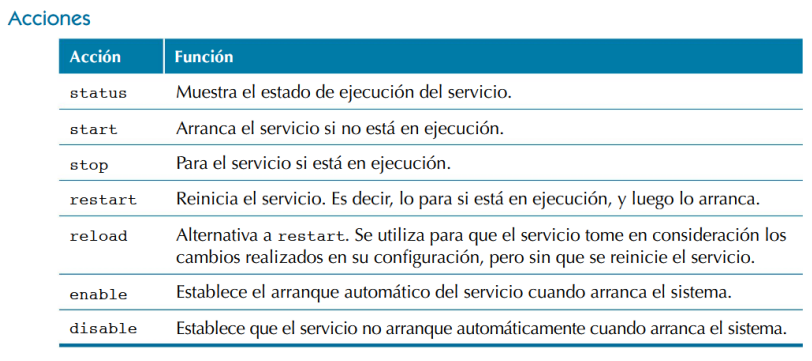
\includegraphics[width=1\linewidth]{img/serviciosLinux.png} 
        \caption{Estados de un proceso.}
    \end{figure}
\end{frame}

\begin{frame}{Servicios en Windows}
    \begin{itemize}
        \item El administrador de servicios permite arrancar y detener servicios.
        \item Permite consultar el estado de ejecución.
        \item Obtener información adicional de dichos servicios.
        \item Configurar el modo de arranque para cada servicio: Automático (arranca automáticamente cuando arranca el SO) o manual.
        \item Presiona Win + R para abrir el cuadro de diálogo "Ejecutar". Escribe services.msc y presiona Enter.
    \end{itemize}
\end{frame}

\begin{frame}{Práctica}
\centering Haz capturas de pantalla de lo que hace cada comando en cada SO.
\end{frame}


\begin{frame}{Hilos}
    \begin{itemize}
        \item Un proceso en ejecución tiene inicialmente un hilo pero podemos crear más de
        forma sencilla.
        \item La ejecución de un proceso termina cuando finaliza la ejecución de todos sus hilos.
        \item Lo mismo a la inversa: Si se termina la ejecución de un proceso se acaba también la
        ejecución de todos sus hilos.
        \item La creación de un nuevo hilo para un proceso ya existente no requiere reservar ni
        inicializar espacio en memoria, ya que dicho espacio es compartido por todos los
        hilos de un mismo proceso.
        \item Si un hilo de un proceso modifica un objeto en memoria, el resto de hilos del mismo
        proceso pueden ver los cambios realizados.
    \end{itemize}
\end{frame}

\begin{frame}
    \begin{itemize}
    \item Cuidado $\to$ Son necesarios mecanismos de sincronización entre hilos para evitar
    problemas que puedan darse si los distintos hilos modifican sin control objetos
    situados en la memoria compartida.
    \item El planificador a corto plazo, gestiona los distintos hilos de un mismo proceso.
    \end{itemize}
\end{frame}

\section{Concurrente, paralela y distribuida}


\begin{frame}{Programación concurrente}

\textbf{Definición}: Implica la ejecución de múltiples tareas (o procesos/hilos) de manera intercalada, en el mismo sistema. Estas tareas parecen ejecutarse al mismo tiempo, pero en realidad, un solo procesador cambia rápidamente de una tarea a otra (multitarea) o varios núcleos ejecutan las tareas en paralelo.

\textbf{Características}:
    \begin{itemize}
        \item Las tareas pueden empezar, ejecutarse y completarse en tiempos diferentes.
        \item Requiere mecanismos de sincronización (como bloqueos, semáforos) para evitar problemas como condiciones de carrera o deadlocks.
        \item No necesariamente se ejecutan al mismo tiempo, pero se solapan temporalmente.
        \item \textbf{Ejemplo}: Un sistema operativo gestionando múltiples aplicaciones abiertas al mismo tiempo.
    \end{itemize}
\end{frame}

\begin{frame}{Programación paralela}
\textbf{Definición}: Se refiere a la ejecución de múltiples tareas de manera simultánea, usualmente en múltiples núcleos de un procesador o en varias máquinas que trabajan en conjunto. A diferencia de la concurrencia, aquí las tareas se ejecutan literalmente al mismo tiempo.

\textbf{Características}:
\begin{itemize}
    \item Requiere que el hardware tenga múltiples núcleos o procesadores para que se pueda dividir el trabajo entre ellos.
    \item Suele ser más eficiente en términos de tiempo de ejecución cuando se aplica a problemas que se pueden dividir en tareas independientes.
    \item \textbf{Ejemplos}: Cálculos científicos de alto rendimiento, procesamiento de gráficos (GPU).
\end{itemize}
\end{frame}

\begin{frame}{Programación distribuida}
\textbf{Definición: }Se refiere a la ejecución de un programa o aplicación en múltiples computadoras (nodos) que están conectadas en red. En este caso, los recursos de hardware (CPU, memoria, almacenamiento) se distribuyen físicamente en diferentes máquinas.


\textbf{Características:}
    \begin{itemize}
        \item Cada nodo tiene su propia memoria y procesador.
        \item Las tareas se comunican entre sí mediante mensajes a través de una red (como internet o una intranet).
        \item Requiere mecanismos para coordinar y sincronizar las tareas distribuidas.
        \item Ejemplos: Aplicaciones en la nube, sistemas de archivos distribuidos (como Hadoop), microservicios, blockchain.
    \end{itemize}
\end{frame}

\section{Profundizando en hilos}

\begin{frame}{Desarrollo de hilos}
    \begin{itemize}
    \item ¿Objetivo principal de lanzar varios hilos de un proceso?
    \item Los distintos hilos de un mismo proceso comparten:
    \begin{itemize}\item El espacio de memoria asignado al proceso.
    \item La información de acceso a ficheros.
    \item Los ficheros no solo se utilizan para almacenar datos. También pueden realizar otras funciones
    como la de controlar dispositivos de E/S.
    \end{itemize}
    \item Sin embargo cada hilo tiene sus propios valores para:
     \begin{itemize}\item Los registros del procesador y contador de programa.
    \item El estado de su pila (stack).
    \begin{itemize}
    \item ¿Qué se guarda en la pila? $\to$ Información referente a las llamadas en curso de ejecución a
    métodos de diversos objetos.
    \item Por ejemplo,entre otras cosas, para cada llamada se guardan los datos locales (en variables
    internas del método)
    \end{itemize}
\end{itemize}
\end{itemize}
\end{frame}
\begin{frame}{Desarrollo de hilos 2}
\begin{itemize}
    \item El intercambio de información es sencillo entre hilos de un mismo proceso, ya que
    comparten la memoria asignada a dicho proceso por el sistema operativo.
    \item Lo complicado será la coordinación de los distintos hilos de un proceso para acceder
    a esos recursos compartidos (contenidos de memoria, ficheros para el control de E/S, ..).
    \end{itemize}
\end{frame}

\begin{frame}
\begin{figure}
        \centering
        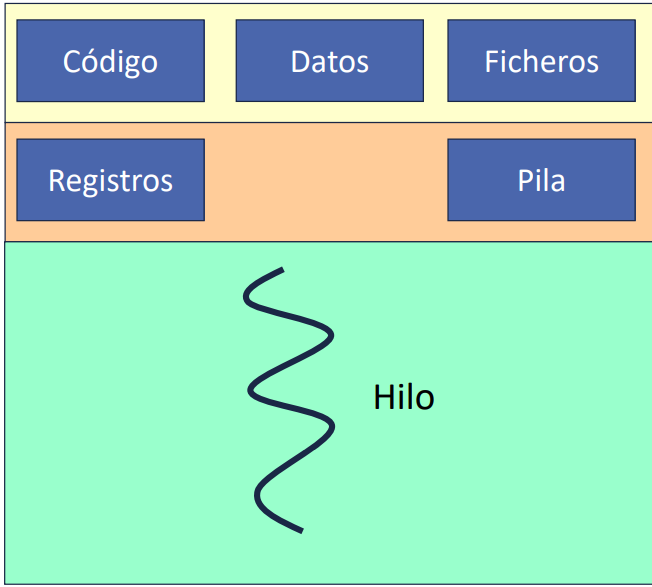
\includegraphics[width=0.65\linewidth]{img/monoHilo.png} 
        \caption{Procesos con un único hilo.}
    \end{figure}
\end{frame}

\begin{frame}
\begin{figure}
        \centering
        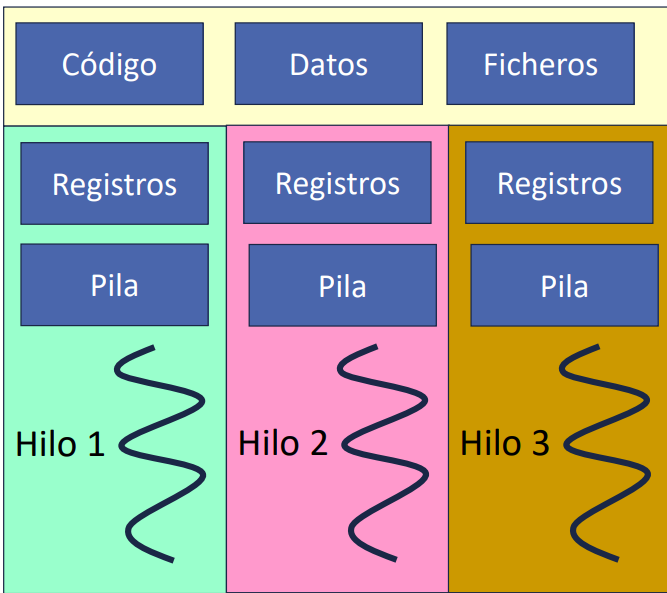
\includegraphics[width=0.65\linewidth]{img/multiHilo.png} 
        \caption{Procesos con varios hilos.}
    \end{figure}
\end{frame}

\begin{frame}{¿Cuándo?}
\begin{itemize}
    \item Programas servidores que proporcionan servicios a otros procesos.
    \item Gracias a los hilos se pueden atender simultáneamente muchas peticiones de servicio y se
    mejora el tiempo de respuesta para ellas.
    \item Programas (de cualquier índole) que muestran una interfaz gráfica de usuario a la
    vez que realizan procesos en segundo plano.
    \item Juegos que disponen de varios elementos que interactúan entre sí y que pueden
    ser controlados por los usuarios.
    \item Programas de control a tiempo real.
    \item Obtención de información del sistema a través de sensores y actuadores.
\end{itemize}
\end{frame}

\begin{frame}{Estados de un hilo}
\begin{figure}
        \centering
        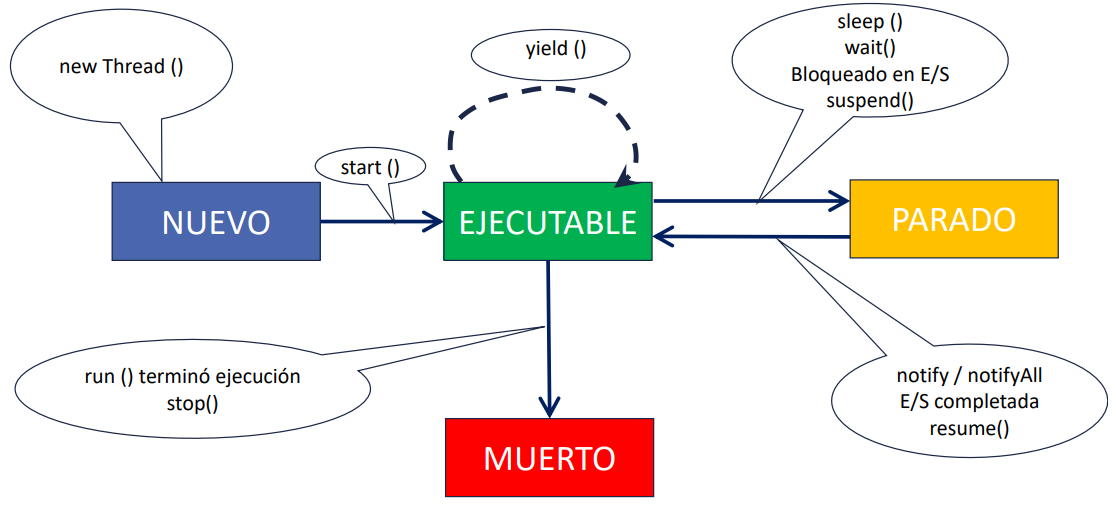
\includegraphics[width=1\linewidth]{img/estadosHilo.png} 
        \caption{Procesos con varios hilos.}
    \end{figure}
\end{frame}

\begin{frame}
    \begin{itemize}
    \item \textbf{Nuevo}
        \begin{itemize}
        \item El hilo creado. Todavía no se ejecuta, pero está preparado.
        \end{itemize}

    \item \textbf{Ejecutable}
        \begin{itemize}
        \item El hilo está preparado para ejecutarse, pero puede estar en ejecución o no dependiendo de si
        el sistema operativo le ha asignado tiempo de CPU. \textbf{No confundir con “en ejecución”.}
        \end{itemize}

    \item \textbf{Muerto}
        \begin{itemize}
        \item Muerte natural tras finalizar su ejecución.
        \item Muerte forzada tras llamar al método correspondiente que produce su muerte.
        \end{itemize}

    \item \textbf{Detenido o parado}
        \begin{itemize}
        \item El hilo está en disposición de poder ejecutarse, pero hay algo que lo evita. Opciones:
        \begin{itemize}
        \item Se ha puesto a dormir (\texttt{wait()}).
        \item Se ha puesto en espera y hasta que otro hilo le notifique lo que necesita.
        \item Lo han suspendido y está en espera de que lo vuelvan a activar.
        \item Está a la espera de que finalice una operación de E/S. 
        \end{itemize}
        \end{itemize}
    \end{itemize}
\end{frame}

\begin{frame}{Debate}
\centering\Large{¿En qué mejoran la programación concurrente con hilos respecto de procesos? ¿Cuándo es más conveniente utilizar una u otra?}
\end{frame}

\end{document}
